\documentclass{article}

\usepackage{amsthm}
\usepackage{amsfonts}
\usepackage{amsmath}
\usepackage{amssymb}
\usepackage{fullpage}
\usepackage{float}

\usepackage{graphicx}

\usepackage[usenames]{color}
\usepackage{hyperref}
  \hypersetup{
    colorlinks = true,
    urlcolor = blue,       % color of external links using \href
    linkcolor= blue,       % color of internal links 
    citecolor= blue,       % color of links to bibliography
    filecolor= blue,        % color of file links
    }
    
\usepackage{listings}

\definecolor{dkgreen}{rgb}{0,0.6,0}
\definecolor{gray}{rgb}{0.5,0.5,0.5}
\definecolor{mauve}{rgb}{0.58,0,0.82}

\lstset{frame=tb,
  language=haskell,
  aboveskip=3mm,
  belowskip=3mm,
  showstringspaces=false,
  columns=flexible,
  basicstyle={\small\ttfamily},
  numbers=none,
  numberstyle=\tiny\color{gray},
  keywordstyle=\color{blue},
  commentstyle=\color{dkgreen},
  stringstyle=\color{mauve},
  breaklines=true,
  breakatwhitespace=true,
  tabsize=3
}

\theoremstyle{theorem} 
   \newtheorem{theorem}{Theorem}[section]
   \newtheorem{corollary}[theorem]{Corollary}
   \newtheorem{lemma}[theorem]{Lemma}
   \newtheorem{proposition}[theorem]{Proposition}
\theoremstyle{definition}
   \newtheorem{definition}[theorem]{Definition}
   \newtheorem{example}[theorem]{Example}
\theoremstyle{remark}    
  \newtheorem{remark}[theorem]{Remark}


\title{Programming Languages Report}
\author{Evelyn Lawrie\\ Chapman University}

\date{\today}

\begin{document}

\maketitle

\begin{abstract}
This report is composed of weekly homework assignments for the Programming Languages course at Chapman University. First, an introduction describes the objectives and contents of this report. Then, further sections explore each assigned problem, week by week. The report ends in a conclusion that summarizes the goals of this project and the larger context it belongs to. 
\end{abstract}

\tableofcontents

\section{Introduction}\label{intro}

This report's goal is to encourage problem solving and original thinking through the implementation of several self-contained weekly homework assignments. The task entails implementing a solution to each problem in a programming language of choice and then working out a given example of the algorithm's logic. By thinking through and thoroughly understanding each step of the algorithm, a deeper understanding of the logic behind why algorithms work the way that they do is cultivated. 

\section{Week 1}

\subsection{GCD Introduction}

The greatest common divisor algorithm can be understood from a geometric, algebraic, and programming perspective. The basis of this algorithm is the idea that whatever divides two numbers n and m where n \textgreater \text{} m must also divide n - m. This can be explored geometrically by visualizing small rectangles dividing up bigger rectangles until there is no smaller common divisor that will evenly fit in rectangles. This algorithm is also referred to as Euclid's algorithm, stemming from the Greek mathematician known as the ``father of geometry" \cite{Gcd}.

When exploring how algebra can solve the greatest common divisor problem, this entails breaking up the problem into three cases: 

\begin{itemize}
\item n \textgreater \text{} m
\item n \textless \text{} m
\item n = m
\end{itemize}

Here is the algebraic definition of Euclid's algorithm using the three cases as described above \cite{Ltx}: 

\begin{equation}
gcd (n, m) = 
\left\{
    \begin{array}{lr}
        gcd(m, m - n), & \text{if } n \text{ } \textgreater \text{ } m\\
        gcd(n, n - m), & \text{if } n \text{ } \textless \text{ } m\\
        n, & \text{if } n = m
    \end{array}
\right\}
\end{equation}

\subsection{GCD Code}

Below is a recursive implementation of the GCD function in Java. 

\begin{lstlisting}
// recursive function to implement the greatest common divisor of two integers
int gcdCalc(int n, int m) {
        if (n > m) {
            return gcdCalc(m, n - m); // subtract m from n when n is bigger 
        }
        else if (n < m) {
            return gcdCalc(n, m - n); // subtract n from m when m is bigger
        }
        else {
            return n; // return n when m and n are equal 
        }
    }
\end{lstlisting}

\subsection{Example Computation}

Below is an implementation of the greatest common divisor algorithm using the example numbers 9 and 33:

\begin{align}
gcd(9, 33) & = gcd(9, 33-9)\\
& = gcd(9, 24)\\
& = gcd(9, 24-9)\\
& = gcd(9, 15)\\
& = gcd(9, 15-9)\\
& = gcd(9, 6)\\
& = gcd(9-6, 6)\\
& = gcd(3, 6)\\
& = gcd(3, 6-3)\\
& = gcd(3, 3)\\
& = 3
\end{align}

\section{Week 2}

\subsection{Towers of Hanoi Introduction}

Towers of Hanoi is a mathematical game in which disks are stacked in ascending order on the far left of three rods. The aim of this puzzle is to move these disks to the far right rod. For each move of one rod at a time, the rule must be obeyed that no disk can be placed onto a disk that is smaller than itself \cite{Wik}. The minimal number of moves required to find a solution given n number of disks is $2^n - 1$ \cite{Wik}.

In the calculation below, \textit{hanoi n x y} is describing a function call to move n disks from rod x to rod y. The far right rod is denoted with a 0, the middle as 1, and the right with a 2. This problem can be approached through recursion, with the function defined as: 

\begin{align}
hanoi \text{ }1 \text{ }x \text{ }y &=  move \text{ }x \text{ }y
\end{align}
\begin{align}
hanoi (n + 1) \text{ }x \text{ }y &=
hanoi \text{ }n \text{ }x \text{ }(other \text{ }x \text{ }y)\\
& move \text{ }x \text{ }y\\
& hanoi \text{ }n \text{ }(other \text{ }x \text{ }y) \text{ }y
\end{align}

The function \textit{move x y} is a function that takes the top disk from position x and moves it to position y. The term \textit{other x y} is the third rod, neither x nor y.

\subsection{Example Computation}

Below are the calculations of the hanoi function with the example of 5 rings moving from left to right: 

\begin{lstlisting}
hanoi 5 0 2  
    hanoi 4 0 1 
        hanoi 3 0 2
            hanoi 2 0 1 
                hanoi 1 0 2 = move 0 2 
                move  0 1
                hanoi 1 2 1 = move 2 1
            move 0 2  
            hanoi 2 1 2
                hanoi 1 1 0 = move 1 0  
                move  1 2  
                hanoi 1 0 2 = move 0 2
        move 0 1
        hanoi 3 2 1
            hanoi 2 2 0 
                hanoi 1 2 1 = move 2 1
                move 2 0
                hanoi 1 1 0 = move 1 0
            move 2 1 
            hanoi 2 0 1 
                hanoi 1 0 2 = move 0 2
                move 0 1
                hanoi 1 2 1 = move 2 1 
    move 0 2 
    hanoi 4 1 2 
        hanoi 3 1 0
            hanoi 2 1 2 
                hanoi 1 1 0 = move 1 0
                move 1 2
                hanoi 1 0 2 = move 0 2 
            move 1 0
            hanoi 2 2 0
                hanoi 1 2 1 = move 2 1
                move 2 0
                hanoi 1 1 0 = move 1 0
        move 1 2
        hanoi 3 0 2 
            hanoi 2 0 1
                hanoi 1 0 2 = move 0 2
                move 0 1
                hanoi 1 2 1 = move 2 1
            move 0 2
            hanoi 2 1 2
                hanoi 1 1 0 = move 1 0
                move 1 2
                hanoi 1 0 2 = move 0 2
\end{lstlisting}

Here are the 31 moves present in the above calculation:

\begin{enumerate}
  \centering
  \item move 0 2
  \item move 0 1
  \item move 2 1
  \item move 0 2
  \item move 1 0
  \item move 1 2
  \item move 0 2
  \item move 0 1
  \item move 2 1
  \item move 2 0
  \item move 1 0
  \item move 2 1
  \item move 0 2
  \item move 0 1
  \item move 2 1
  \item move 0 2
  \item move 1 0
  \item move 1 2
  \item move 0 2
  \item move 1 0
  \item move 2 1
  \item move 2 0
  \item move 1 0
  \item move 1 2
  \item move 0 2
  \item move 0 1
  \item move 2 1
  \item move 0 2
  \item move 1 0
  \item move 1 2
  \item move 0 2
\end{enumerate}

\subsection{Towers of Hanoi Formula}

The word \textit{hanoi} appears 31 times in the computation above. This is the same frequency as the number of moves per n amount of disks. Therefore, the formula for amount of function calls necessary for the computation of a given number of disks is: 


\begin{align}
numFunctionCalls(numDisks) = numMoves(numDisks) = 2^{numDisks} - 1
\end{align}

\section{Week 3}

\subsection{Parsing Introduction}

Concrete syntax is defined as written code while abstract syntax is the representation of code, which is what the code means to the machine. Abstract syntax can be visualized with trees, and it is made up of algebraic/recursive data types. Parsing is the process of translating concrete syntax into abstract syntax. Some programming languages skip the parsing step and are composed of abstract syntax rather than concrete syntax. Parsing analyzes symbols using a parser generator to see whether they follow formal grammar rules, like the ones outlined by BNFC or other formal grammar structures. 

\subsection{Concrete Syntax Trees}

Given the context-free grammar: 

\begin{lstlisting}
Exp -> Exp '+' Exp1 
Exp1 -> Exp1 '*' Exp2              
Exp2 -> Integer            
Exp2 -> '(' Exp ')'  
Exp -> Exp1             
Exp1 -> Exp2 
\end{lstlisting}

The task is to implement concrete syntax trees for the example strings given. The grammar above is a set of rules that defines a language. In this case, that language is the set of arithmetic expressions using times and plus. Below are the written out parse trees:

\begin{figure}[H]
\begin{center}
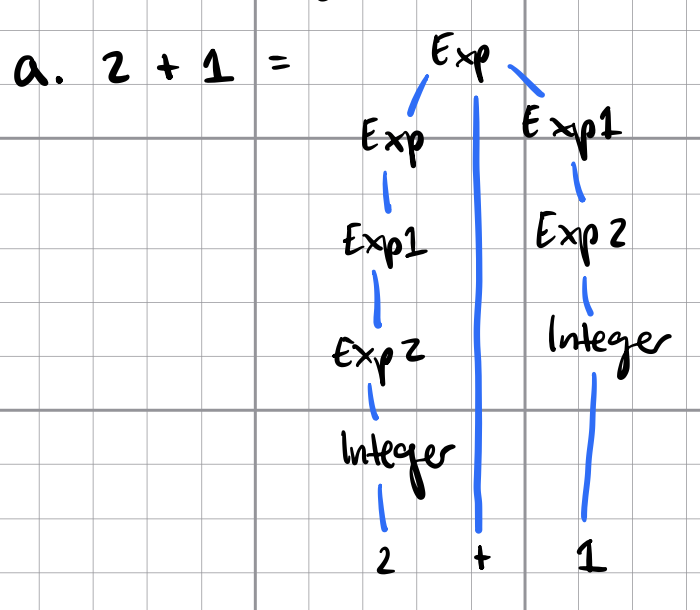
\includegraphics[scale=0.4]{img/C1.png}
\end{center}
\caption{2 + 1}\label{C1}
\end{figure}

\begin{figure}[H]
\begin{center}
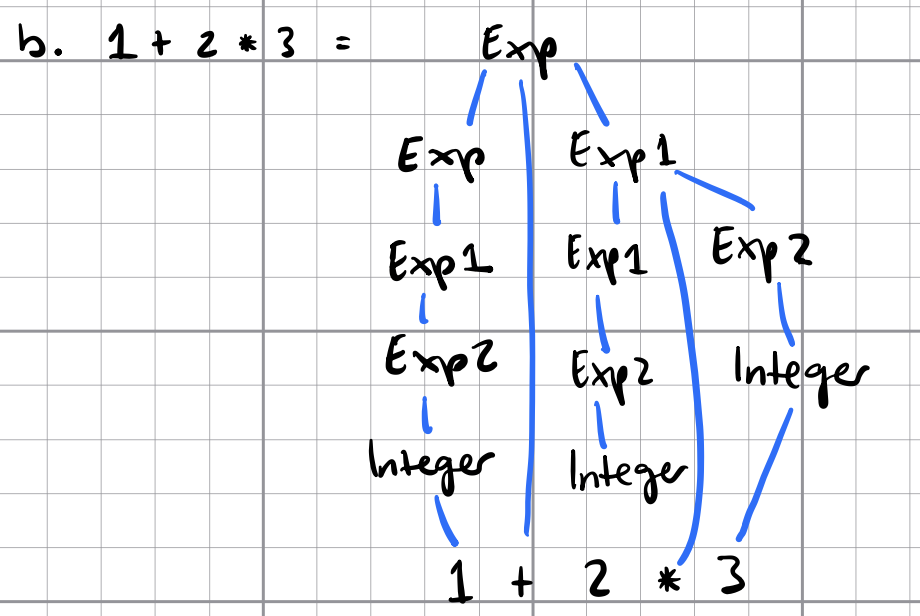
\includegraphics[scale=0.4]{img/C2.png}
\end{center}
\caption{1 + 2 * 3}\label{C2}
\end{figure}

\begin{figure}[H]
\begin{center}
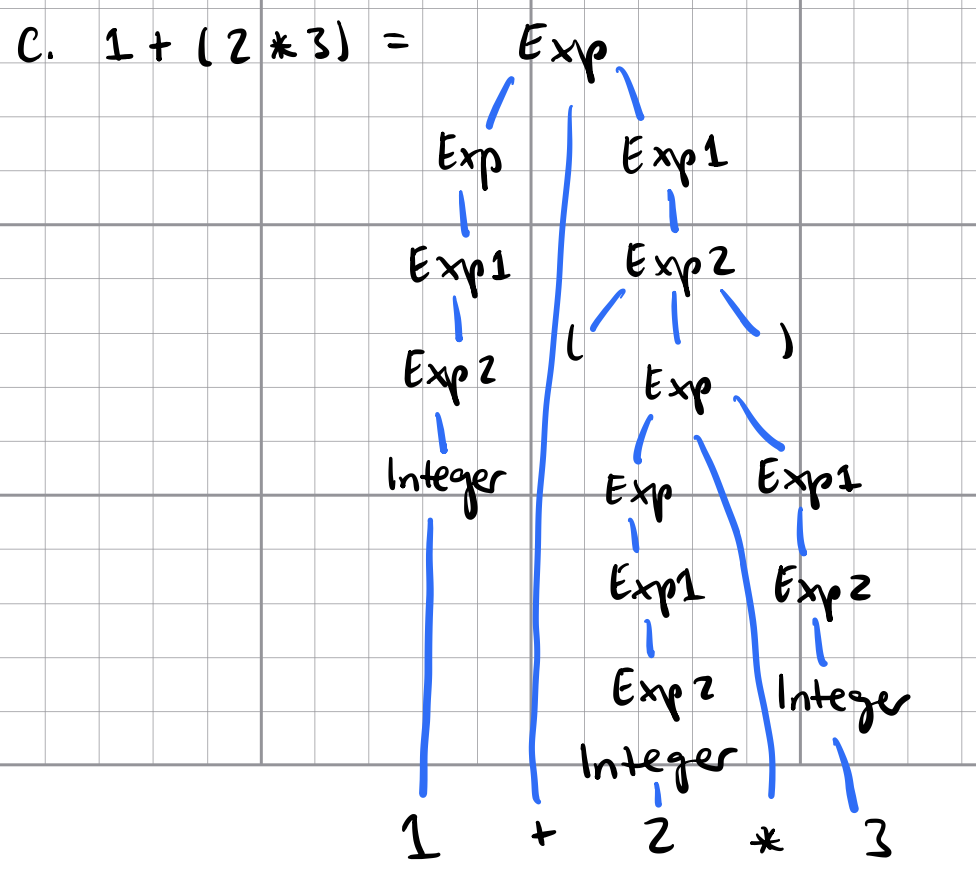
\includegraphics[scale=0.4]{img/C3.png}
\end{center}
\caption{1 + (2 * 3)}\label{C3}
\end{figure}

\begin{figure}[H]
\begin{center}
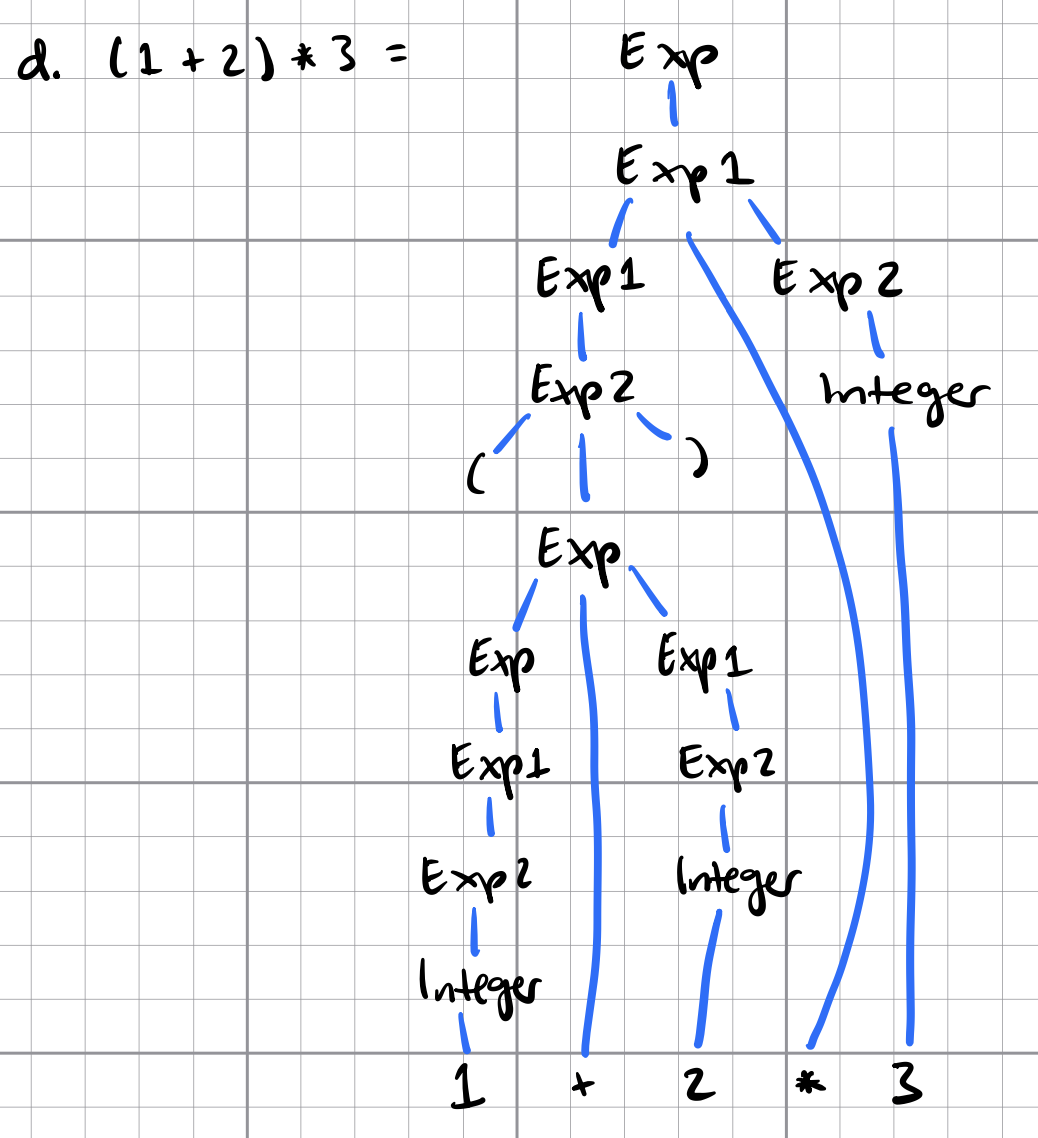
\includegraphics[scale=0.4]{img/C4.png}
\end{center}
\caption{(1 + 2) * 3}\label{C4}
\end{figure}

\begin{figure}[H]
\begin{center}
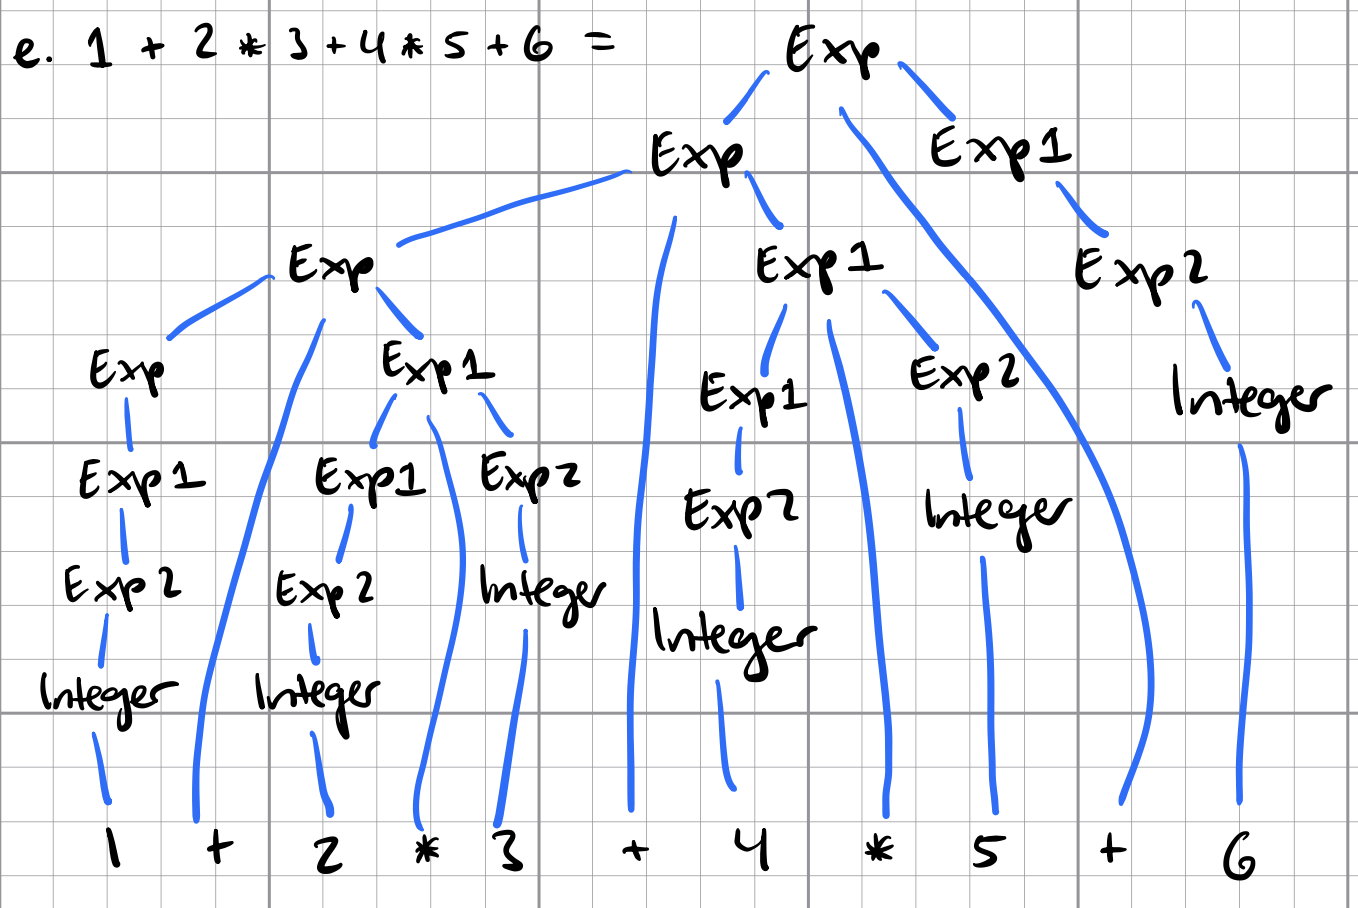
\includegraphics[scale=0.4]{img/C5.png}
\end{center}
\caption{1 + 2 * 3 + 4 * 5 + 6}\label{C5}
\end{figure}

\subsection{Abstract Syntax Trees}

Given the BNFC grammar: 

\begin{lstlisting}
Plus.   Exp ::= Exp "+" Exp1 ;
Times.  Exp1 ::= Exp1 "*" Exp2 ;
Num.    Exp2 ::= Integer ;
	
coercions Exp 2 ;
\end{lstlisting}

We are tasked with writing out the abstract syntax trees for the example arithmetic equations that follow the rules of the BNFC grammar defined above. BNFC comes with its own language, LNBF, which is a language for writing context-free grammars. The above set of rules is an example of what grammar looks like in BNFC and it represents the structure for the set of arithmetic equations that use plus and times. The following trees are written as abstract syntax trees. These trees differ from concrete syntax trees in three ways: the unnamed rules are eliminated, parent nodes are labeled with the names of the corresponding rules, and concrete syntax (such as symbols like "+" or "*") are eliminated. 

\begin{figure}[H]
\begin{center}
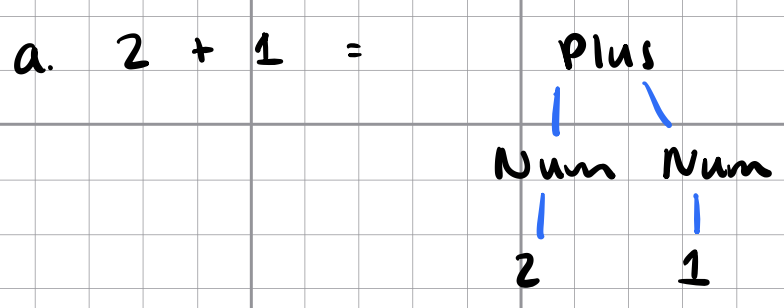
\includegraphics[scale=0.4]{img/A1.png}
\end{center}
\caption{2 + 1}\label{A1}
\end{figure}

\begin{figure}[H]
\begin{center}
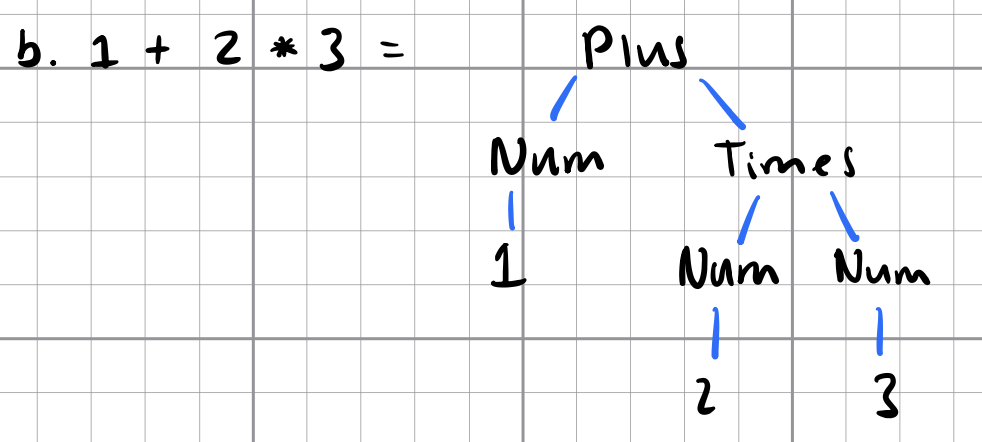
\includegraphics[scale=0.4]{img/A2.png}
\end{center}
\caption{1 + 2 * 3}\label{A2}
\end{figure}

\begin{figure}[H]
\begin{center}
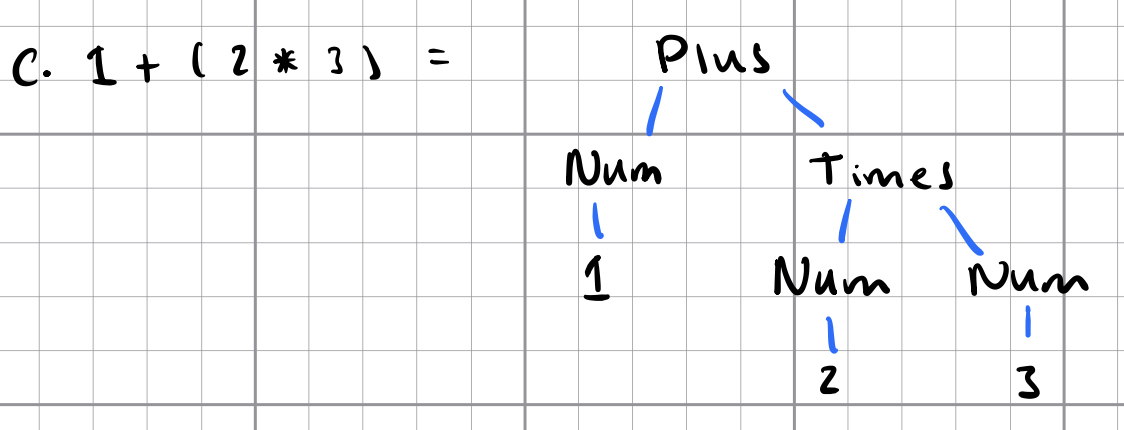
\includegraphics[scale=0.4]{img/A3.png}
\end{center}
\caption{1 + (2 * 3)}\label{A3}
\end{figure}

\begin{figure}[H]
\begin{center}
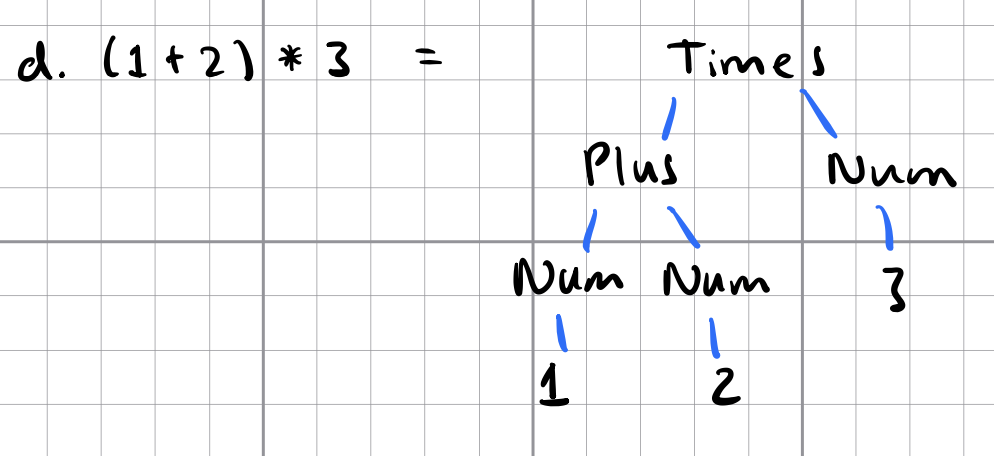
\includegraphics[scale=0.4]{img/A4.png}
\end{center}
\caption{(1 + 2) * 3}\label{A4}
\end{figure}

\begin{figure}[H]
\begin{center}
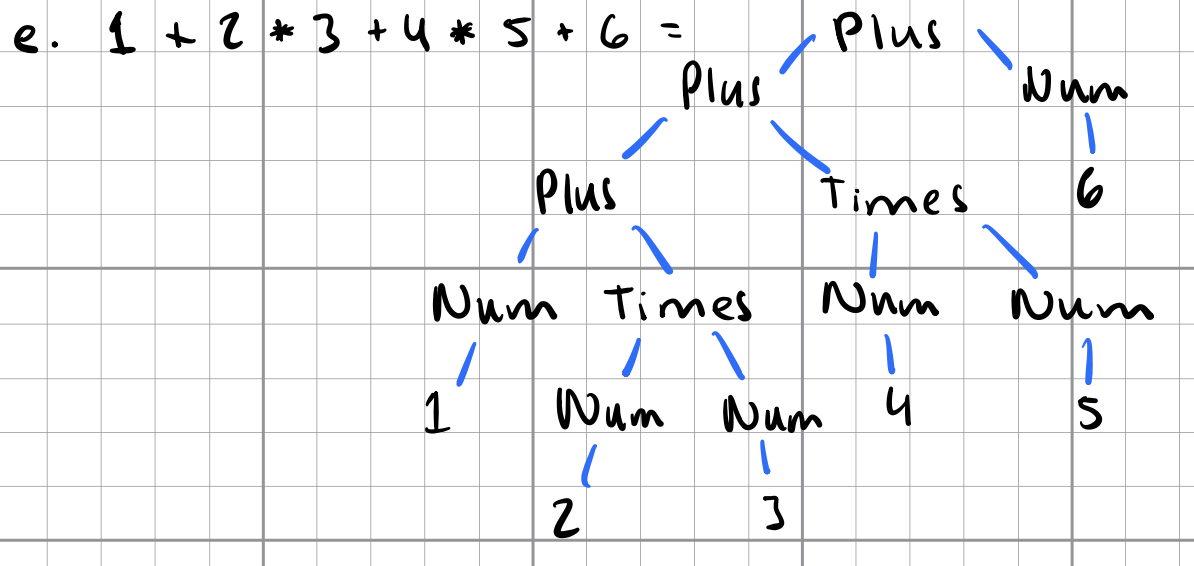
\includegraphics[scale=0.4]{img/A5.png}
\end{center}
\caption{1 + 2 * 3 + 4 * 5 + 6}\label{A5}
\end{figure}

Since parenthesis are not taken into account when writing out the nodes of abstract syntax trees, the tree for the equation $1+2*3$ is identical to the one for the equation $1+(2*3)$. The first equation follows the order of operations, in which multiplication is evaluated before addition. The second tree puts parenthesis around the multiplication terms, which visually illustrates which part of the equation to evaluate first, even though the equation is evaluated the same without the parenthesis given the order of operations. $(1+2)*3$ manipulates the order of operations, causing the addition to be evaluated first and therefore diverging from the calculation of the first equation without any parenthesis. 

\section{Week 4}

\subsection{Lambda Calculus Introduction}

Lambda calculus only has three programming constructs. These are abstraction, application, and variables. According to abstraction, a program called $e$ containing the variable $x$ will look like $\lambda x. e$ in Lambda calculus. Application outlines how if $e1$ and $e2$ are programs, $e1 e2$  is the program that applies the function $e1$ to argument $e2$. Finally, the most basic programs in Lambda calculus only consist of variables. Lambda calculus abstracts away a lot of the syntax used in most other programming languages. The report this week focuses on the syntax and semantics of Lambda calculus.

\subsection{Syntax}

For the syntax portion of this week's homework, we are tasked with using the grammar of BNFC outlined for Lambda calculus to output the linearized abstract syntax trees from the following expressions, as well as manually write out the abstract syntax trees for them. Below are the calculations for the given Lambda calculus expressions: 

\begin{figure}[H]
\begin{center}
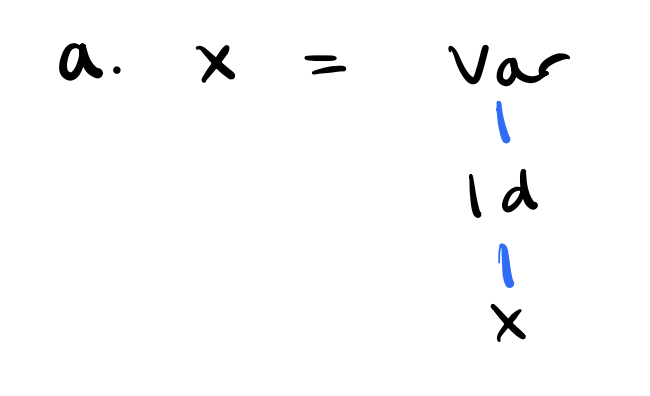
\includegraphics[scale=0.4]{img/aAST.png}
\\
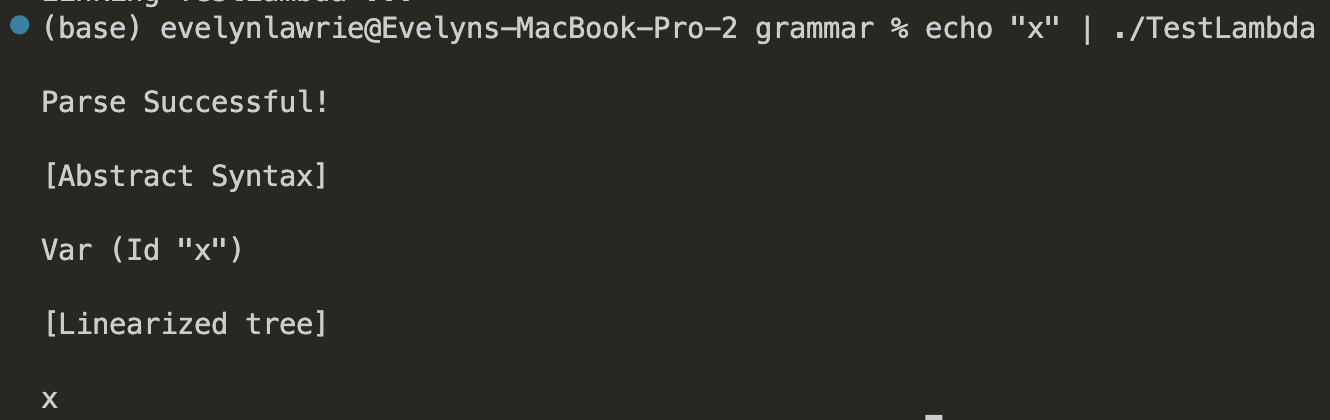
\includegraphics[scale=0.4]{img/ASTa.png}
\end{center}
\caption{x}\label{ASTa}
\end{figure}

\begin{figure}[H]
\begin{center}
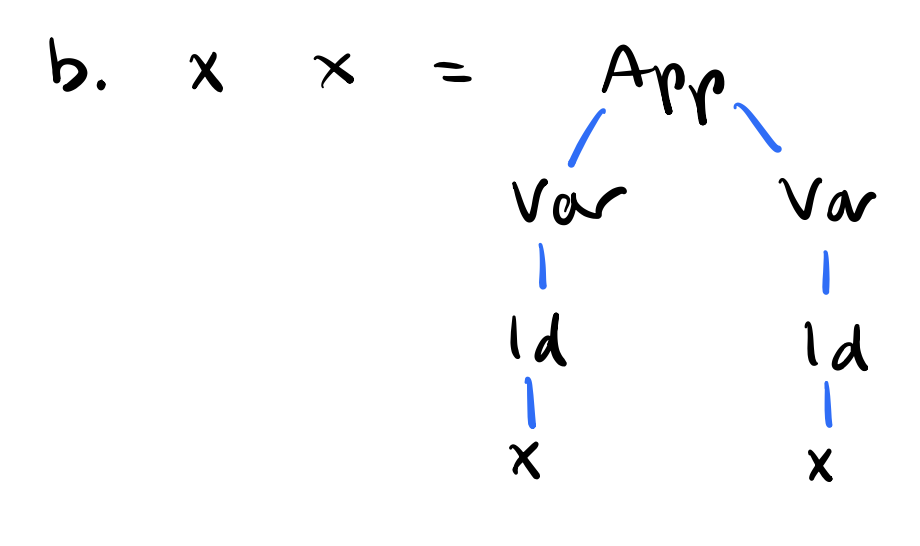
\includegraphics[scale=0.4]{img/bAST.png}
\\
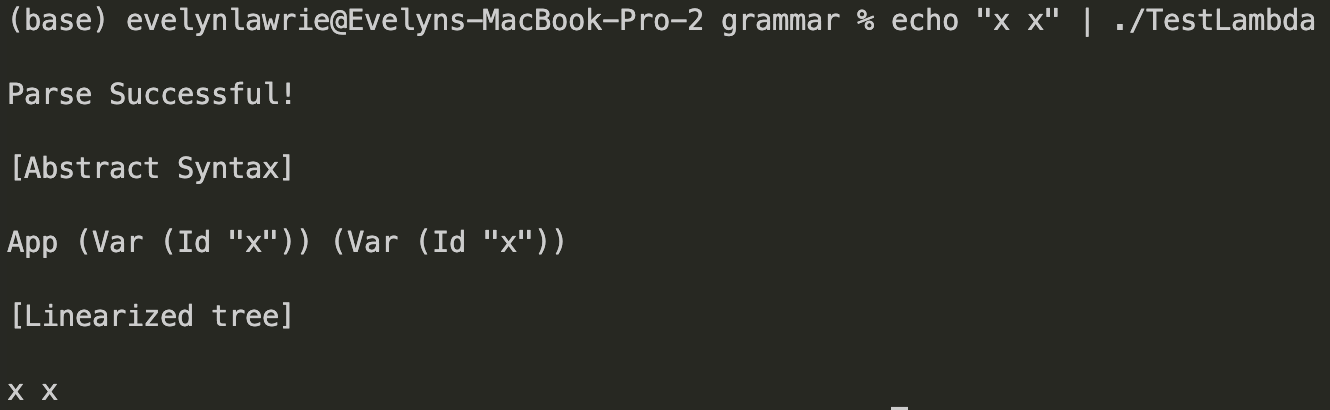
\includegraphics[scale=0.4]{img/ASTb.png}
\end{center}
\caption{x x}\label{ASTb}
\end{figure}

\begin{figure}[H]
\begin{center}
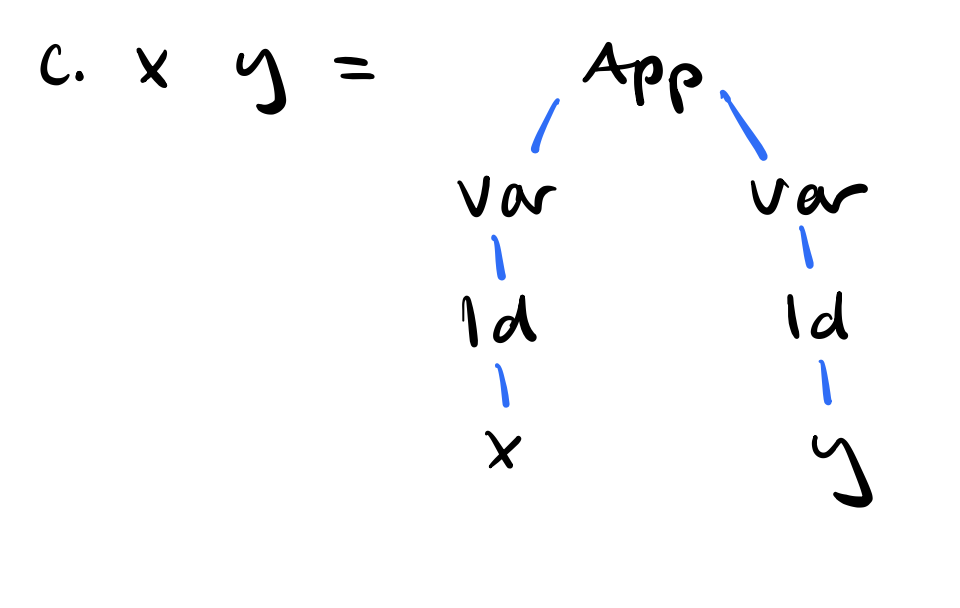
\includegraphics[scale=0.4]{img/cAST.png}
\\
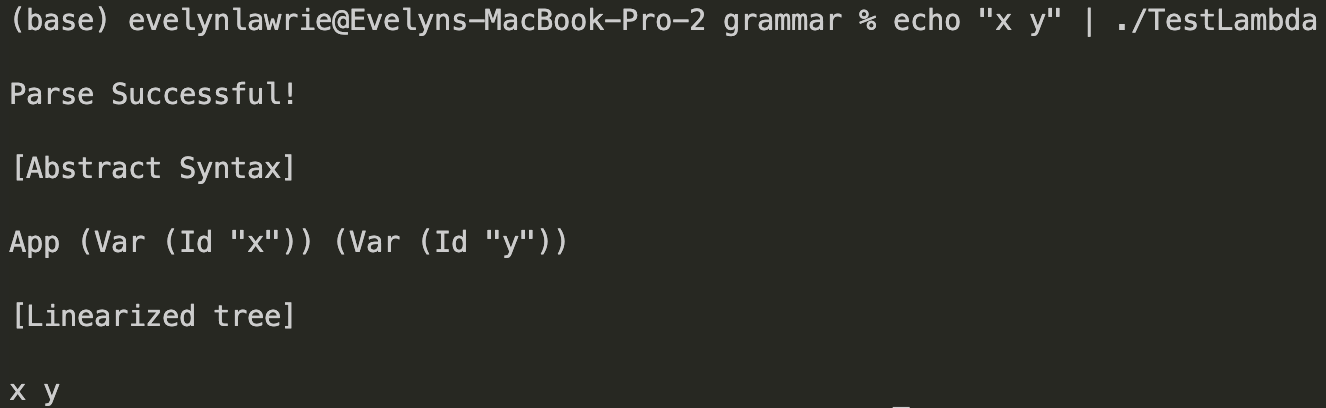
\includegraphics[scale=0.4]{img/ASTc.png}
\end{center}
\caption{x y}\label{ASTc}
\end{figure}

\begin{figure}[H]
\begin{center}
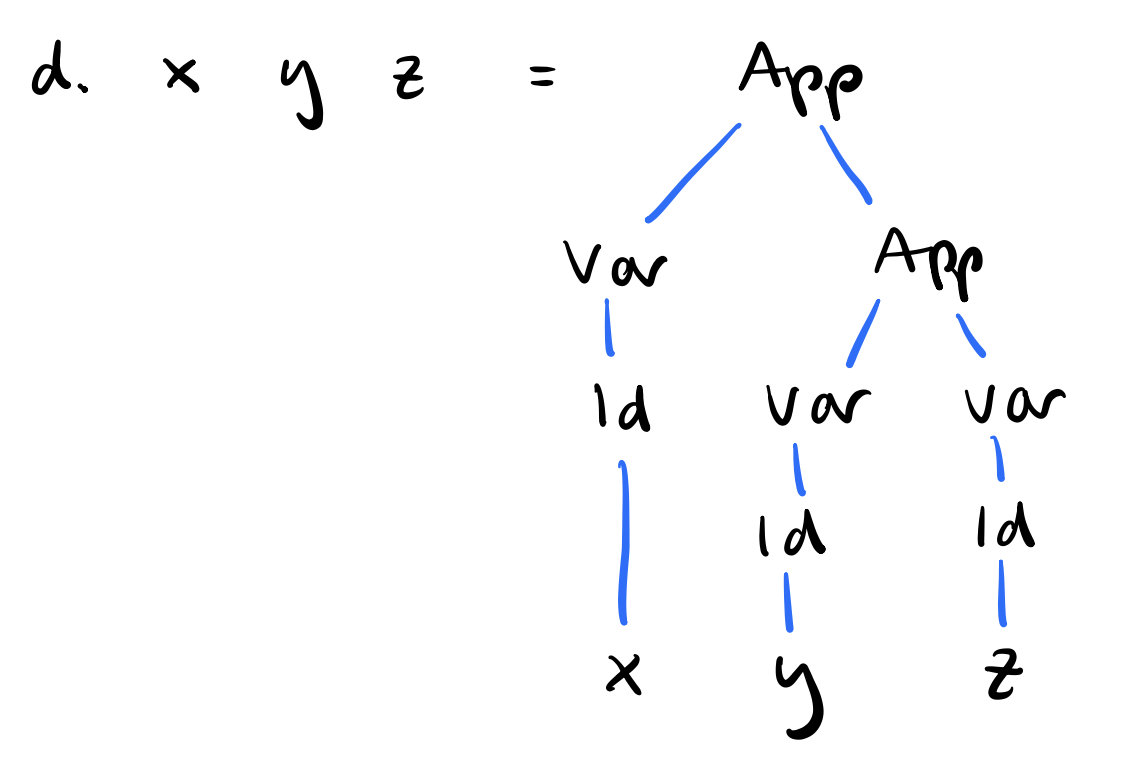
\includegraphics[scale=0.4]{img/dAST.png}
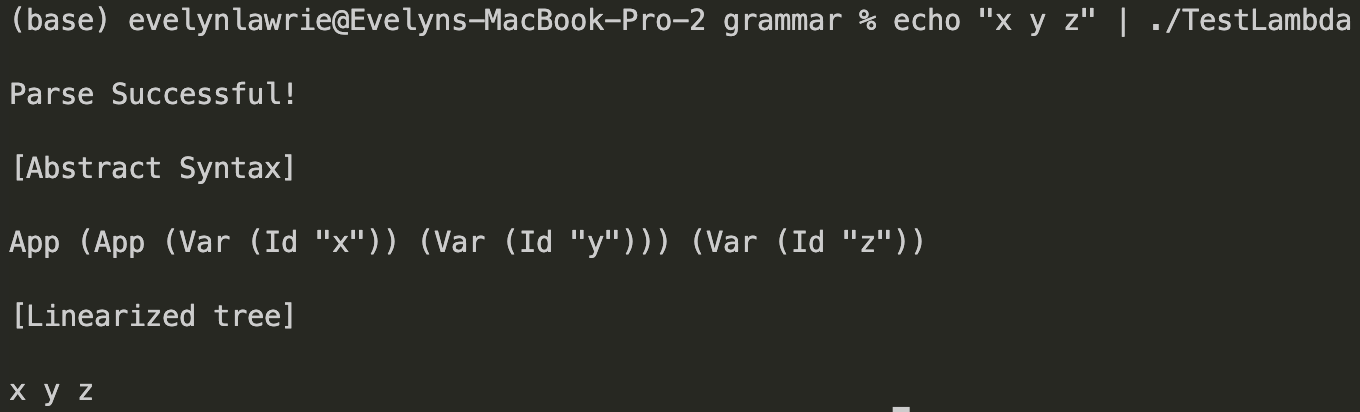
\includegraphics[scale=0.4]{img/ASTd.png}
\end{center}
\caption{x y z}\label{ASTd}
\end{figure}

\begin{figure}[H]
\begin{center}
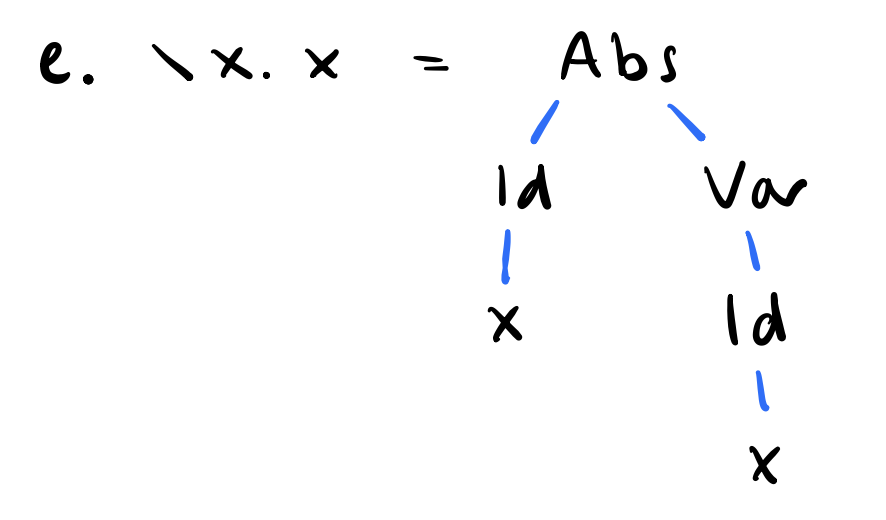
\includegraphics[scale=0.4]{img/eAST.png}
\\
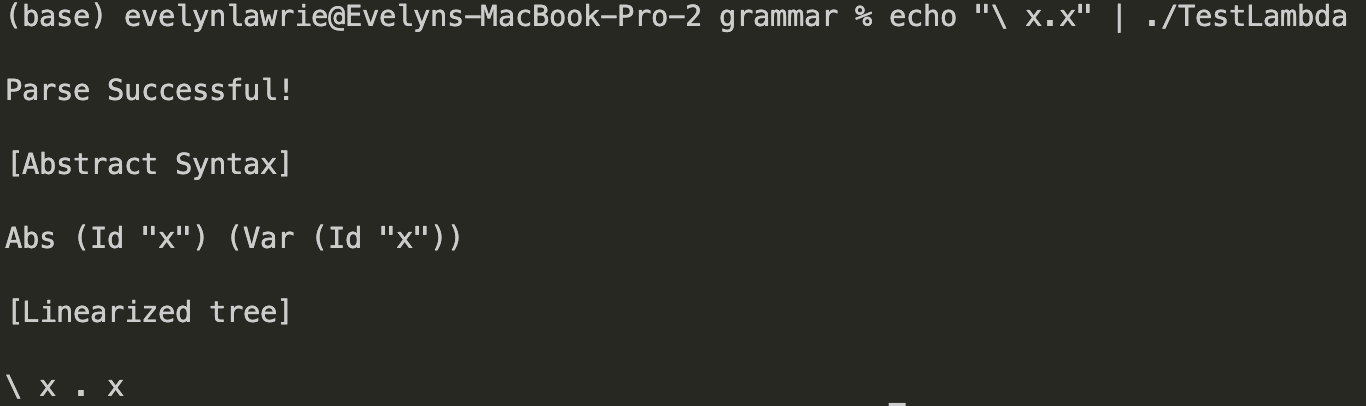
\includegraphics[scale=0.4]{img/ASTe.png}
\end{center}
\caption{$\lambda x. x$}\label{ASTe}
\end{figure}

\begin{figure}[H]
\begin{center}
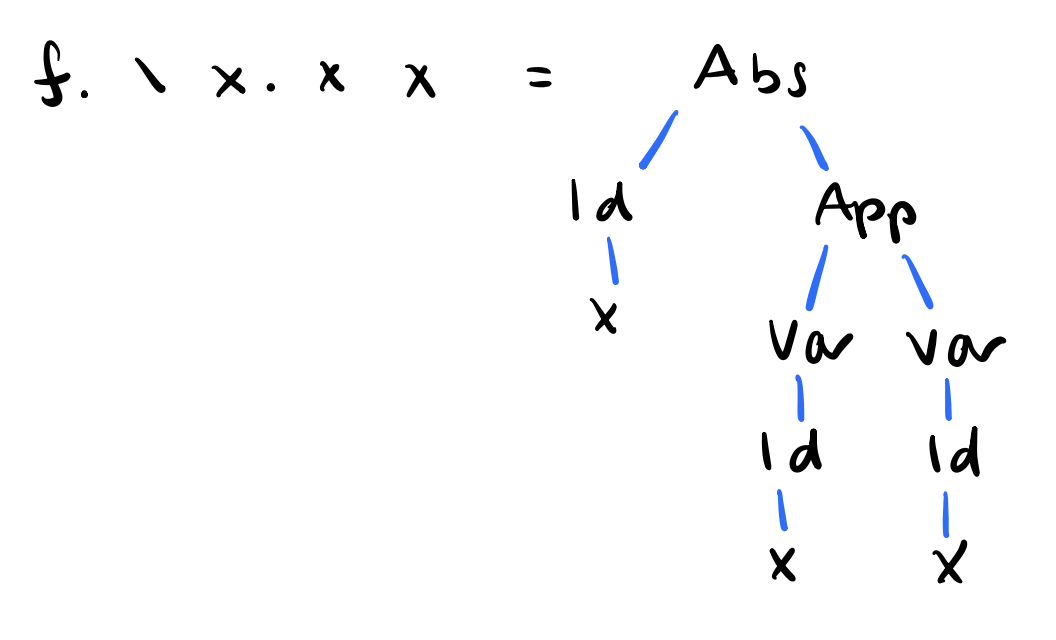
\includegraphics[scale=0.4]{img/fAST.png}
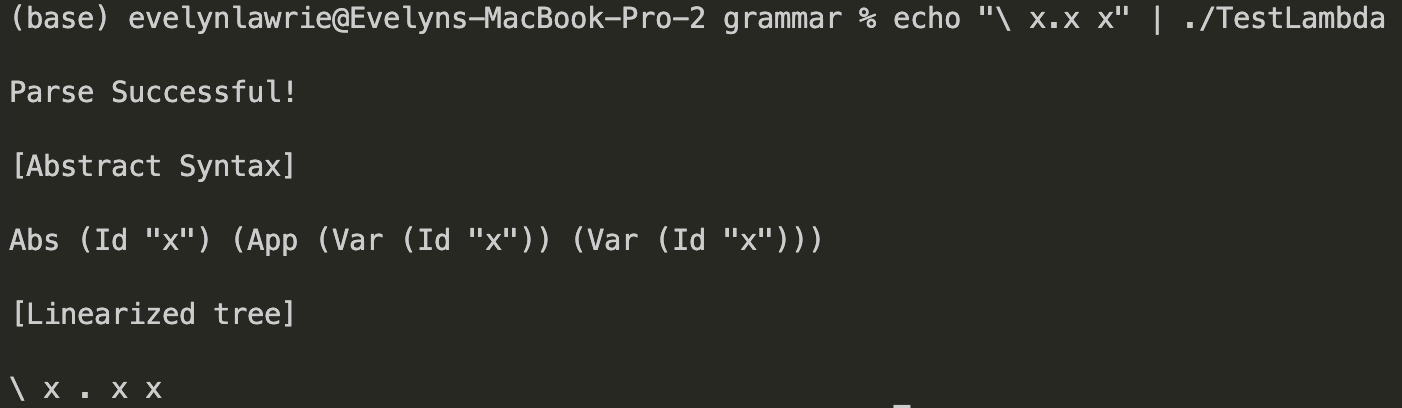
\includegraphics[scale=0.4]{img/ASTf.png}
\end{center}
\caption{$\lambda x. x x$}\label{ASTf}
\end{figure}

\begin{figure}[H]
\begin{center}
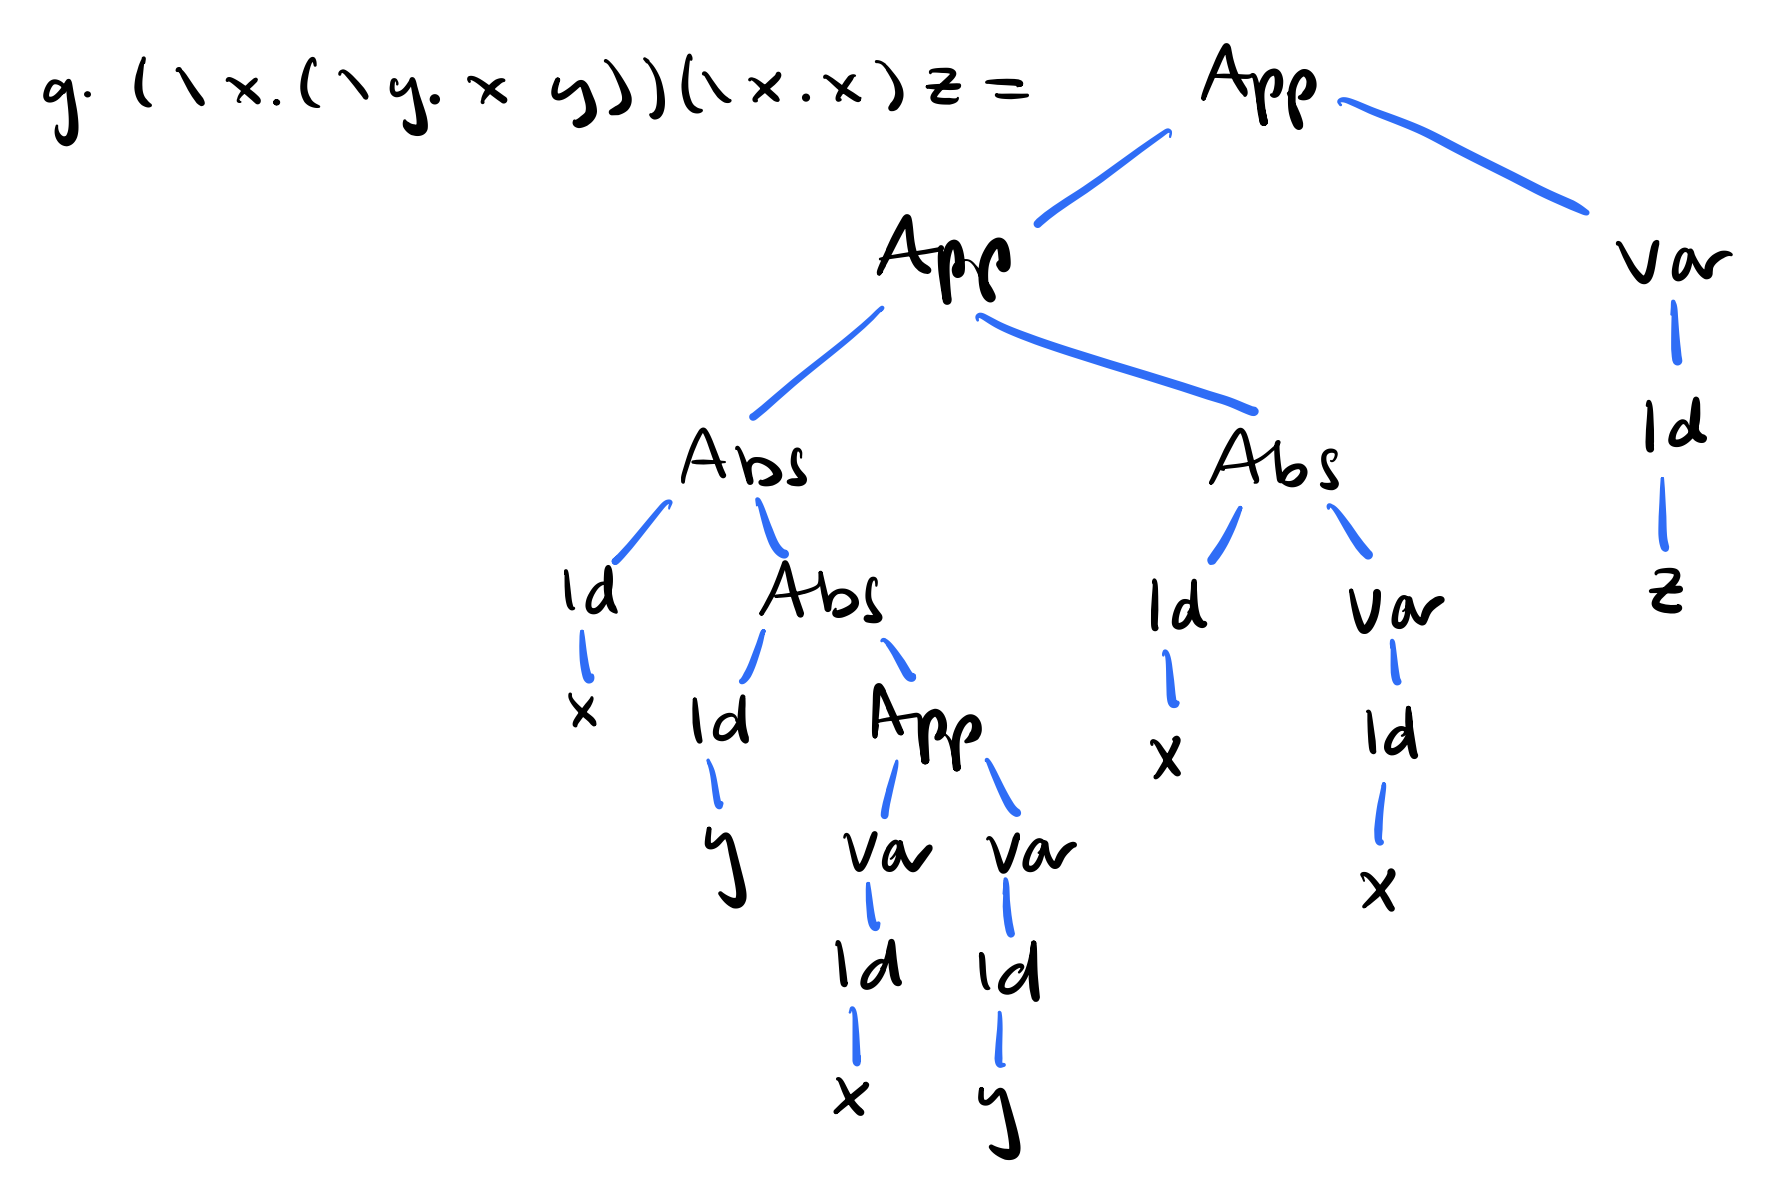
\includegraphics[scale=0.4]{img/gAST.png}
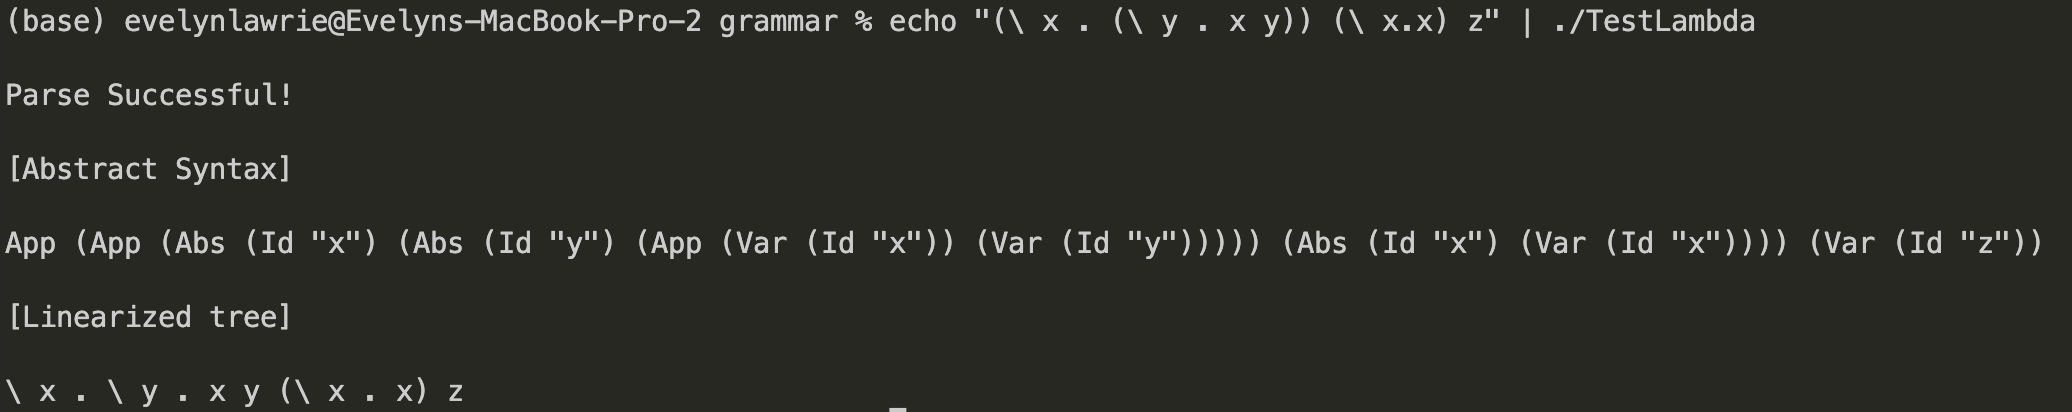
\includegraphics[scale=0.4]{img/ASTg.png}
\end{center}
\caption{$(\lambda x. (\lambda y. x y)) (\lambda x. x) z$}\label{ASTg}
\end{figure}

\begin{figure}[H]
\begin{center}
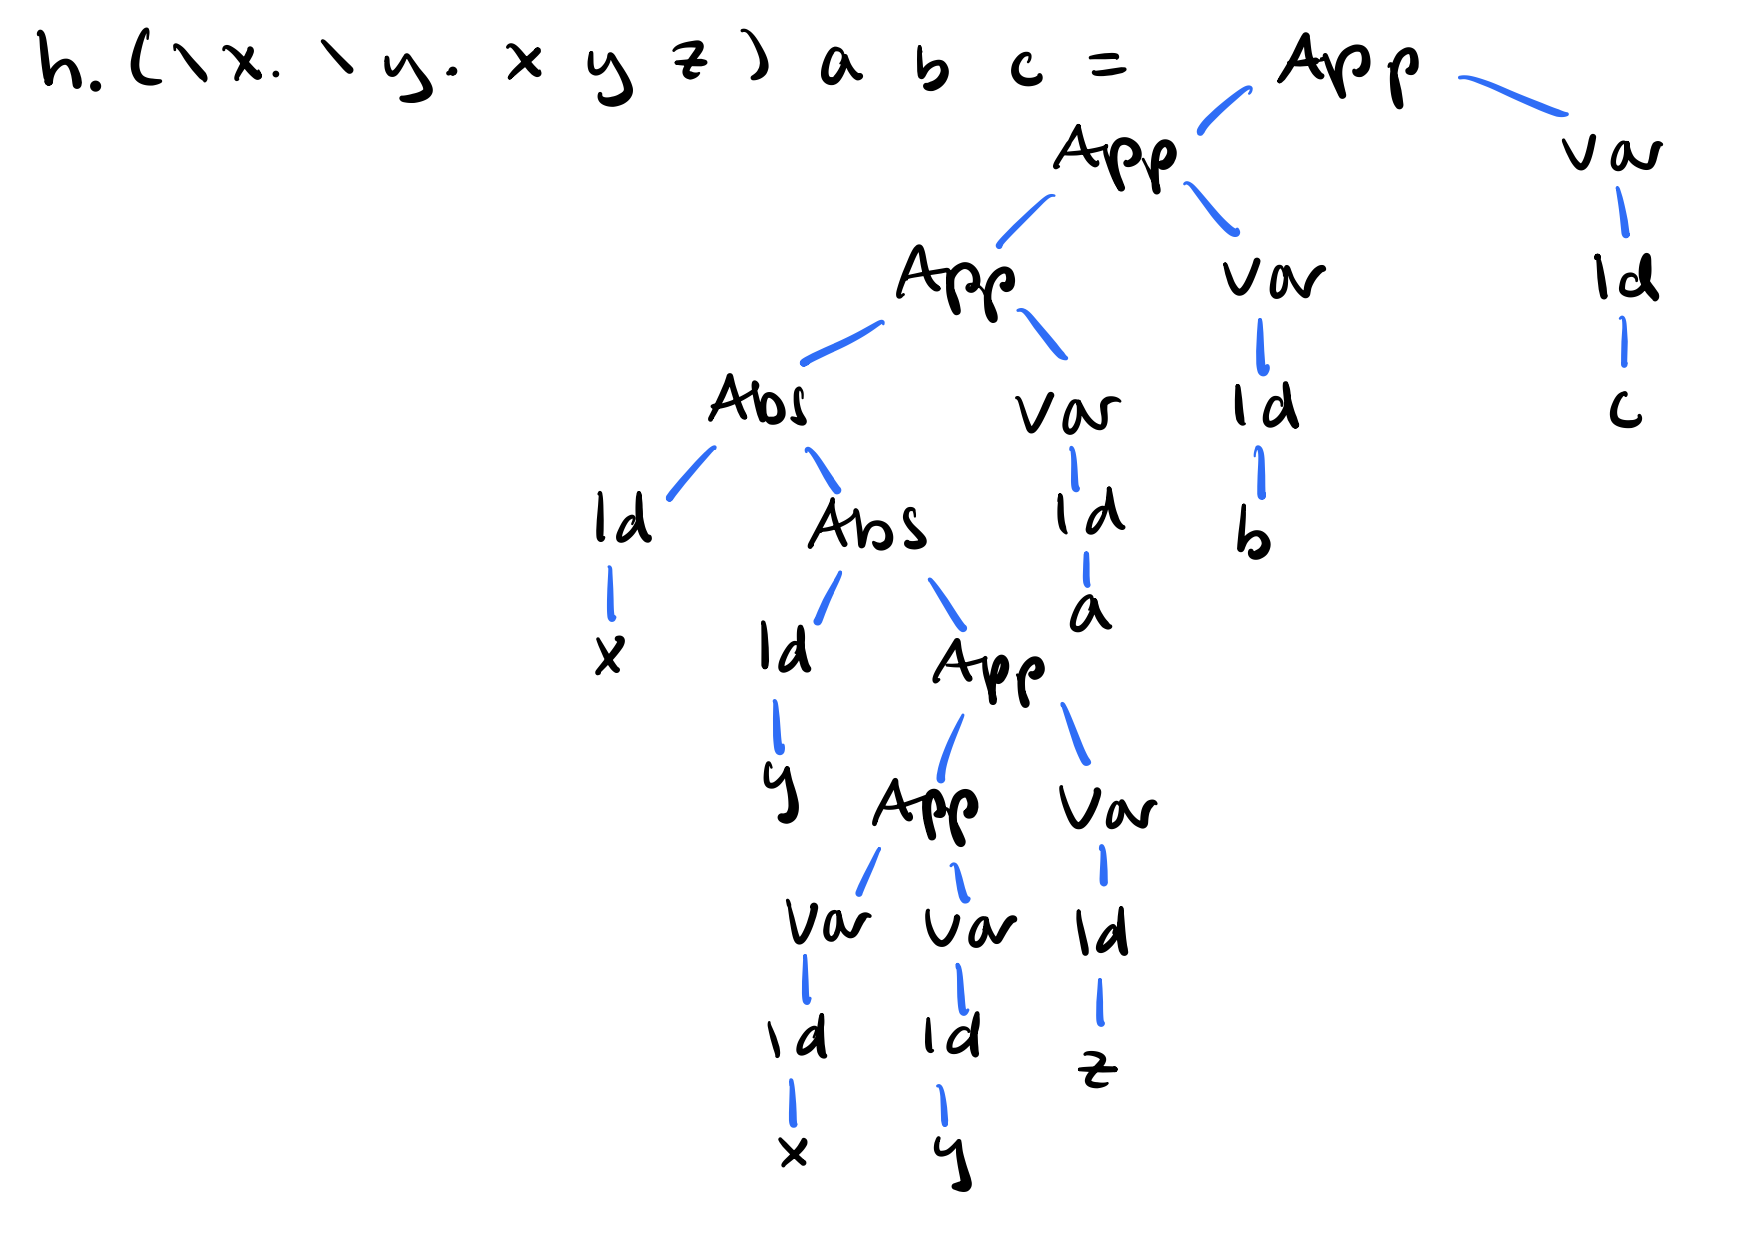
\includegraphics[scale=0.4]{img/hAST.png}
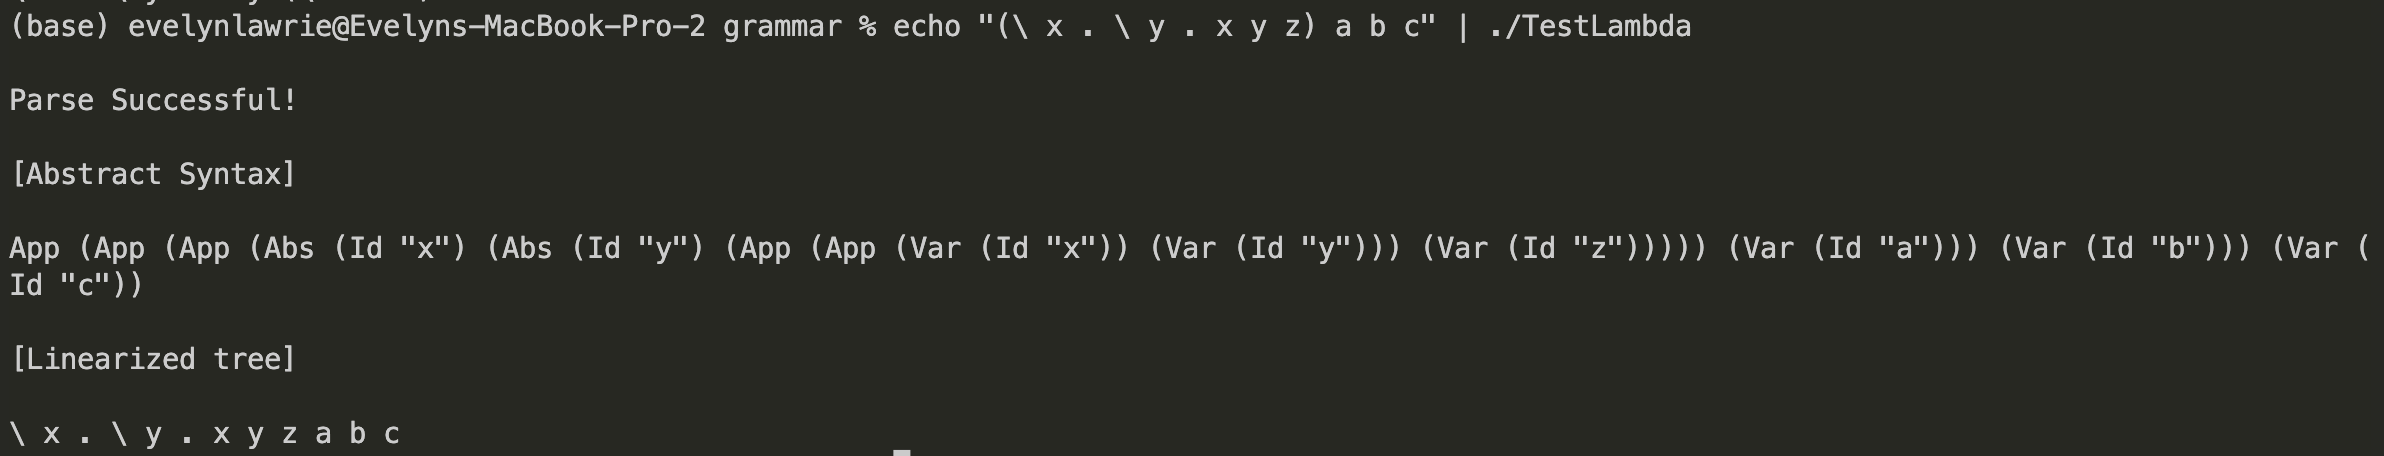
\includegraphics[scale=0.4]{img/ASTh.png}
\end{center}
\caption{$(\lambda x. \lambda y. x y z) a b c$}\label{ASTh}
\end{figure}

\subsection{Semantics}

The Lambda calculus semantics homework entails finishing the workout that we started in class. Below is an image of my typed out computation: 

\begin{figure}[H]
\begin{center}
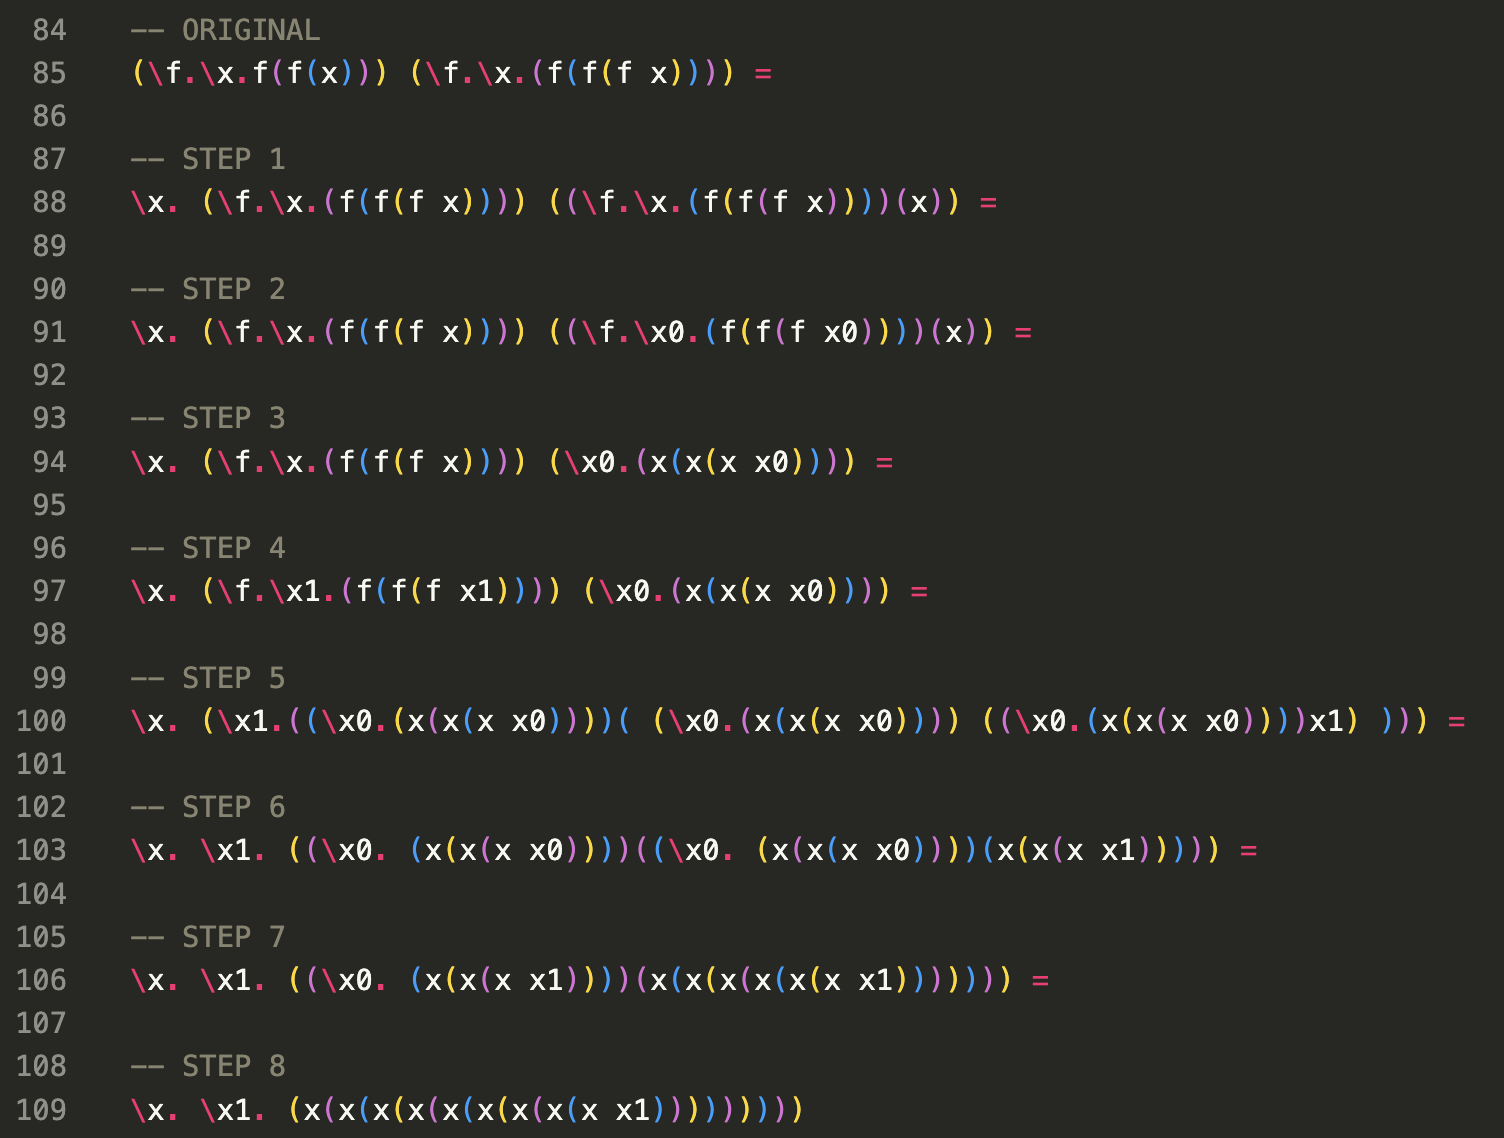
\includegraphics[scale=0.6]{img/workoutSolution.png}
\end{center}
\caption{Workout Solution}\label{WS}
\end{figure}

\section{Lessons from the Project}

Recursion is the basis for many of these weekly projects. Understanding in detail how recursion works behind the scenes aids in the implementation of the coded solutions in this report. Recursion is a problem-solving technique that utilizes the call stack to create functions that call other functions, or more simplified versions of themselves, within them. To visualize and fully understand the structure of recursive calls, it is best to draw out the problem as a tree data structure, with each recursive call being a node of the tree. Every time a base case is reached, that node becomes a leaf and then the branches are explored upwards from there, branching off when needed and computing calculations from the bottom up. This is describing depth-first search, in which one branch of the tree is explored all the way until reaching a base case. This process is repeated for the whole tree, usually starting at the left and moving right. Parsing, rewriting strings into trees, is a method of visualizing how a computer executes a certain computation and can be vital in the comprehension of the recursion problems explored in this report. 

Another key takeaway that improves upon the concept of recursion is memoization. This deals with the repeated nodes or function calls within a function's tree. With simple recursion, it is common for the same calculation to be computed multiple times, which decreases efficiency of the code. This creates exponential run times which can prove highly costly for large computations. The process of memoization stores values that the function has already computed in a hash table or similar data structure for easy lookup and avoidance of unnecessary repeated calculations. The recursive function call then implements a quick lookup in this data structure (constant runtime) and extracts the output if the current input value has already been calculated. If the current parameter has not been calculated, it performs the regular calculations and then stores the new value inside of the memo object. The process of memoization greatly decreases the time complexity of recursive functions, in the majority of cases bringing it down from an exponential to a polynomial or linear type runtime. This problem-solving technique stood out to me as a highly important lecture topic that serves as a way to optimize the algorithms presented in this report.

From Week 2's addition to this report, the syntax that displays the example computation is designed to illustrate how the stack grows and shrinks with recursive function calls. The stack grows from left to right until a base case is reached, shrinking from there going right to left. Working through this example thoughtfully can aide in the understanding of how recursive functions are interacted with on the stack. We are able to visualize through the Towers of Hanoi problem what the call stack looks like behind the scenes and why recursive functions work the way that they do. Recursion is the basis for many of the computations explored throughout this course, making a thorough understanding of its implementation crucial in fully absorbing its key takeaways. 

Additionally, parsing is an important topic in this class, as it is an essential process that machines employ when evaluating most computer code. Computers parse concrete syntax into abstract syntax, which is then evaluated by the virtual machine, using the model of computation. This process is something we will encounter daily as computer programmers. Better understanding how a computer parses and understands the information we give it can make us more efficient programmers. Being able to decipher parse trees given a context-free grammar and examples of its language allows us to better understand how computers process code. BNFC and other types of parser generators define rules that the computer follows when interpreting concrete syntax strings. Approaching computer programs in terms of language and grammar teaches us to interpret programs logically and think of parsing as something that follows strict rules and does not take semantics into account. The way humans read and interpret programs is very different from how computers parse them, and we as programmers have to keep in mind that what the computer sees is taken at face value and evaluated according to the rules we have defined. This teaches us to be explicit and straightforward with how we program, avoiding ambiguity and confusion.

Week 4 gives us an introduction to Lambda calculus and its applications. Lambda calculus is the simplest possible programming language. The syntax may look very different to most programming languages, but it contains all of the same concepts. This allows us to strip back a lot of the syntax and get to the root of the basis of programming languages. To be able to write programs using only variables, abstraction, and application is a good starting point to understand the logic of why computer programs work the way that they do. Using variable binding and substitution for Lambda calculus computations (using the Alpha and Beta rules) teaches us how to rename formal parameters and perform capture avoiding substitution, which are the building blocks of Lambda calculus. In capture avoiding substitution, we rename the formal parameters (bound variables) and then replace that parameter in the body of the function by the argument. Reducing Lambda calculus expressions according to these rules demonstrates how this logic is computed by the machine in its simplification. We are able to better understand how computers interpret code by working step-by-step through these computations and having a foundational understanding of Lambda calculus as a whole. 

\section{Conclusion}\label{conclusions}

This report details various logical problems and their solutions implemented throughout this semester. As illustrated in this report, these algorithms can be approached in various different ways. Exploring different approaches to the same problem hones the skill set of novel solution creation, which allows programmers to complete tasks by thinking outside of the box in ways that seem less than straightforward. The thought processes behind the solutions to these problems can be applied to technical interviews, future computer science courses, and projects assigned in the workplace within the field of computer programming. The problem-solving techniques developed in this class and through this report serve as a basis of knowledge to assist students with our future endeavours. 

\begin{thebibliography}{99}
\bibitem[LTX]{Ltx} \href{https://latex-tutorial.com/piecewise-functions-latex/}{Cases and piecewise functions in LaTex}, LaTex-Tutorial.com, 2023.
\bibitem[GCD]{Gcd} Alexander Kurz, \href{https://www.youtube.com/watch?v=ZcJMj0antos}{gcd and Euclid's algorithm}, YouTube, 2020.
\bibitem[WIK]{Wik} \href{https://en.wikipedia.org/wiki/Tower_of_Hanoi}{Tower of Hanoi}, Wikipedia, 2023.
\end{thebibliography}

\end{document}
